\chapter{Results and Evaluation}
\label{ch:results}

\section{Evaluation protocol}
\label{sec:protocol}

Evaluation runs through the eot-bench harness on the French subset: 400 turns and
1{,}054 silences, of which 400 are ends of turn and 654 are holds. Each of those silences is one micro-pause in the sense of
Section~\ref{sec:realtime}: one moment at which the system must decide. The harness sweeps
the endpointing policy and reports two measures. Per-span AUC says how well a model tells a
silence that ends a turn from one that is only a pause. The latency and cut-in frontier says
how long the system waits, and how often it speaks over a caller who has not finished. 

Take one silence that ends a turn and one that
does not. The per-span AUC is the probability that the model scores the first higher. 0.5 is
a coin flip, 1.0 is a perfect ordering. All lexical and fusion figures are cross-validated with folds split by call,
so no call appears in both training and test.

One methodological point conditions the comparisons. Three of the systems decide as the transcript
arrives: the streaming recognisers Soniox, AssemblyAI and OpenAI GPT-Realtime 2. They cannot
be scored on per-span AUC, because they score at a different moment from the one evaluated
here. Their latency is reported and their AUC left out, since the number would not be
comparable. 

\section{Fusion against the acoustic baseline}
\label{sec:fusionresults}

Table~\ref{tab:fusion} gives AUC and latency, the latter at a 5\,\% and then a 10\,\%
cut-in budget.

\begin{table}[H]
\centering
\caption[Fusion results on the French benchmark]{Fusion results on the public French
benchmark (eot-bench, 1{,}054 silences). \emph{Benchmark-fitted} means the lexical head was
fitted on the benchmark itself, cross-validated with folds split by call;
\emph{medical-fitted} means the lexical model was fine-tuned on Tennor medical French and
applied here unchanged. The lexical branch was scored per span but never run through the policy sweep on its own,
so it carries no latency figure. TF-IDF is term frequency-inverse document frequency, STT is
speech-to-text.}
\label{tab:fusion}
\begin{tabular}{@{}lccc@{}}
\toprule
Model & AUC & Latency @ 5\,\% & @ 10\,\% \\
\midrule
Acoustic only (Smart Turn v3) & 0.814 & 873\,ms & 608\,ms \\
Lexical only (benchmark-fitted) & 0.845 & --- & --- \\
\midrule
Fusion, medical-fitted lexical & 0.789 & 850\,ms & 659\,ms \\
Fusion, benchmark-fitted TF-IDF & 0.872 & 759\,ms & 548\,ms \\
\textbf{Fusion, benchmark-fitted CamemBERT} & \textbf{0.897} & \textbf{715\,ms} & \textbf{510\,ms} \\
\midrule
ultraVAD & 0.817 & 846\,ms & 613\,ms \\
LiveKit v1-mini (commercial) & 0.884 & 798\,ms & 541\,ms \\
Deepgram Flux (commercial) & 0.915 & 676\,ms & 353\,ms \\
LiveKit v1 (commercial) & 0.937 & 635\,ms & 376\,ms \\
Soniox (streaming STT) & n/a & 557\,ms & 463\,ms \\
\bottomrule
\end{tabular}
\end{table}

Fusion lifts the AUC from 0.814, for the acoustic model, to 0.897: a gain of 0.083. That is the comparison the objectives are stated against,
but not the whole picture. The lexical branch alone reaches 0.845, so what fusion adds over
the better of its two inputs is 0.052, not 0.083. The first number says what the deployed system
would gain, the second whether combining the signals beats taking the stronger one.

A gain is only a contribution if it can be shown statistically, so the data was resampled
by call, three thousand times. The 95\,\% confidence interval on
the gain is $[0.063, 0.104]$; no resample produced a non-positive gain, so $p < 1/3000$, which is the finest bound three
thousand resamples can support. Resampling by
call rather than by silence matters, because silences from one call are not
independent and treating them as such would inflate the significance. The gain is not noise.

The fitted weights are worth reporting, since Section~\ref{sec:fusionform} claims
interpretability as a reason for choosing this form. Averaged over the five folds they are
$w_0 = -3.59$, $w_{\mathrm{ac}} = 1.95$, $w_{\mathrm{lex}} = 4.29$ and
$w_{\mathrm{inter}} = 1.22$, with a standard deviation across folds of at most $0.21$. The
lexical branch therefore carries about $2.2$ times the weight of the acoustic one, which
agrees with the two branches scored separately and is the opposite of what the framing of
this project assumed.

The bottom of the table sets the condition under which fusion helps at all. The lexical
signal only helps when it is in distribution. The medical-fitted model, applied to the
generic French of the benchmark, degrades the decision to 0.789, below the acoustic baseline
it was meant to improve. Fusion
is not beneficial in itself. It is beneficial on condition that the lexical model matches
the data, and that condition bounds where this method can be deployed.

The comparison against the other systems needs care. The table adds ultraVAD, an
open-source detector that scores on audio alone, like Smart Turn. At 0.817 it edges past the
acoustic baseline. That is worth recording, because it is the only comparator here that is
neither commercial nor part of this project. At 0.897 the fusion sits above it and above
LiveKit v1-mini (0.884), but below Deepgram Flux (0.915) and LiveKit v1 (0.937). It does not
beat the strongest commercial detectors on AUC, and the margin against v1-mini is too small
to claim a win there either.

On latency it trails as well: 715\,ms against 557\,ms for Soniox and 635\,ms for LiveKit v1
at a 5\,\% budget. Deciding at a micro-pause rather than as the text arrives is a real cost,
and a deliberate consequence of not blocking on transcription
(Section~\ref{sec:nonblocking}). It is not the whole explanation, though: two of the three
streaming services are slower still, AssemblyAI at 822\,ms and GPT-Realtime 2 at 837\,ms.

Figure~\ref{fig:pareto} extends the two budgets of the table to the whole frontier.
The fusion curve sits below the acoustic one across the entire range, so the gain is not an
artefact of the operating points chosen for reporting. It also sits above the LiveKit curve
throughout, so neither is the shortfall.

\begin{figure}[H]
\centering
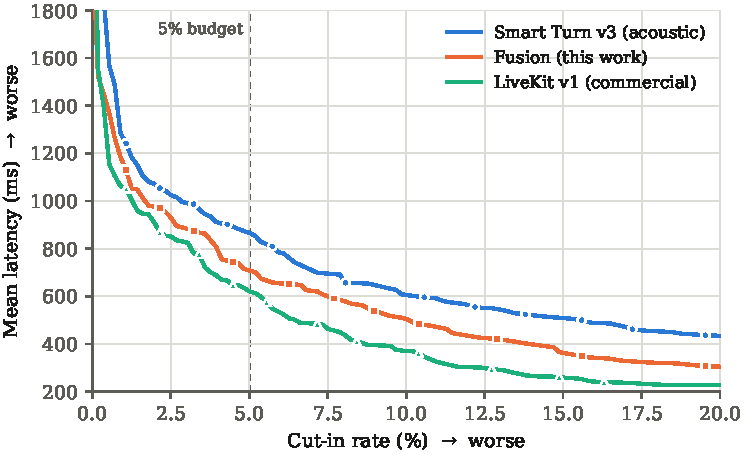
\includegraphics{figures/fig_pareto.pdf}
\caption[Latency against cut-in frontier]{Swept latency-versus-cut-in frontier on the
French benchmark. Lower and to the left is better. The dashed lines mark the 5\,\% and 10\,\% cut-in budgets quoted in
Table~\ref{tab:fusion}.}
\label{fig:pareto}
\end{figure}

\section{Where the gain comes from}
\label{sec:hardcase}

The project is motivated by three cases where silence is a poor cue: a name being spelled
out, digits given in blocks, a pause on a date. It seemed worth checking whether the gain
actually lands on those cases. Each silence was tagged from the causal caller text preceding it, and the AUC recomputed
within each subgroup (Table~\ref{tab:hardcase}).

\begin{table}[H]
\centering
\caption[Per-case breakdown]{Per-case breakdown on the French benchmark. Subgroup sizes
are given first because several groups are far too small to support inference: the spelling
and date rows rest on six and four spans, so their AUCs are reported for completeness only
and no weight is placed on them. Only the digit and plain-text rows are large enough to
compare.}
\label{tab:hardcase}
\begin{tabular}{@{}lrrrcc@{}}
\toprule
Case & $n$ & eot & hold & AUC acoustic & AUC fusion \\
\midrule
Spelling & 6 & 1 & 5 & 0.800 & 1.000 \\
Digits & 269 & 107 & 162 & 0.825 & 0.875 \\
Date & 4 & 2 & 2 & 1.000 & 1.000 \\
Plain text & 764 & 290 & 474 & 0.807 & 0.901 \\
Empty transcript & 11 & 0 & 11 & n/a & n/a \\
\midrule
All & 1{,}054 & 400 & 654 & 0.814 & 0.897 \\
\bottomrule
\end{tabular}
\end{table}

The first of the two findings runs against the framing of this project. On the digit case, which is large
enough to trust at $n = 269$, fusion gains 0.050; on ordinary text it gains 0.094. The motivating case is the one where the lexical signal helps \emph{least}.

That is explicable in hindsight: a partially dictated number is lexically ambiguous in a way an
unfinished sentence is not, because nothing in the words themselves says whether more
digits are coming. The hard cases stay hard, and the bulk of the headline gain comes from
ordinary utterances.

The second is about the benchmark rather than the method itself. Spelling appears six times in
1{,}054 silences and dates four times. Generic French, as sampled here, essentially does not
contain the phenomena that make medical intake difficult, so the public benchmark cannot
test the case the project exists for. This is an argument for in-domain evaluation, not
against it, and it is the reason Section~\ref{sec:gold} matters even though its result is
negative.

\section{Calibration}
\label{sec:calibresults}

Table~\ref{tab:ece} gives the expected calibration error of Equation~\ref{eq:ece}, before
and after post-hoc isotonic recalibration, measured on a held-out split.

\begin{table}[H]
\centering
\caption[Expected calibration error]{Expected calibration error, raw and after post-hoc
isotonic recalibration on a held-out split. Every external system that can be scored at the
evaluation point is listed; nothing is selected. The raw column is the probability each
system actually emits, and the calibrated column is what an integrator can reach by
correcting it, which is available to every row equally.}
\label{tab:ece}
\begin{tabular}{@{}lcc@{}}
\toprule
Model & ECE (raw) & ECE (calibrated) \\
\midrule
Smart Turn v3 & 0.216 & 0.079 \\
ultraVAD & 0.108 & 0.071 \\
LiveKit Turn Detector v1 & 0.091 & 0.052 \\
Deepgram Flux & 0.087 & 0.083 \\
LiveKit Turn Detector v1-mini & 0.084 & 0.051 \\
\midrule
\textbf{This work (fusion)} & \textbf{0.064} & 0.043 \\
\bottomrule
\end{tabular}
\end{table}

The three streaming services are excluded here. An expected calibration error pairs a
predicted probability with the outcome of the same span, which is exactly the pairing
Section~\ref{sec:protocol} rejects for their AUC; reporting one while refusing the other
would be inconsistent. One figure from those excluded runs is worth quoting, not as a result but as evidence for
the exclusion itself: sampled at the evaluation point, GPT-Realtime 2 falls from an ECE of
0.374 to 0.007 under recalibration. A collapse that large is what a near-constant score
looks like, and a system that has not yet decided emits exactly that. No row is given for it
in Table~\ref{tab:ece}.

This chapter treats ECE $> 0.05$ as miscalibrated. The line is a working convention, not a
standard. All five external detectors that can be scored at the evaluation point fall above
it, as do ten of the eleven runs in the span set.
\texttt{calibration\_study.py} in the submitted corpus prints every run.

Before any correction, the fused probability is the best calibrated of the set, at 0.064
against 0.084 for the nearest external system. That is the comparison that bears on
deployment, since none of these systems ships a recalibration step and an integrator
therefore gets the raw column. The margin should not be pressed. v1-mini, Deepgram Flux and LiveKit v1 are all within 0.03,
the table rests on a single held-out split of 214 spans, and no interval is attached to any
of these values. The ordering among the four leading systems is not a result this
dissertation can defend.

The calibrated column does not favour this work. Recalibration needs only a held-out split,
so any integrator can apply it to any row. Applied uniformly it compresses the range:
v1-mini reaches 0.051 and LiveKit v1 0.052 against 0.043 here. The ordering survives, the
distance does not. Across all eleven runs the best-calibrated is this project's own
dialogue-context variant at 0.039, which Section~\ref{sec:negative} reports as a failure on
every other measure. The finding this section supports is therefore about the field and not
about a ranking: miscalibration is universal, correcting it is cheap, and nobody does it.
Nor does that spare this work, which sits uncorrected at 0.064, above the same line.

The mechanism is the one described in Section~\ref{sec:calibration-lit}: these are neural classifiers trained to
discriminate. Nothing in a discriminative objective rewards a probability that matches a
frequency, and the leaderboard never asks for one. 

The consequence is practical. A threshold
placed on a probability that does not correspond to a real frequency cannot be connected to
a cost, and every one of these systems exposes a threshold to its users as though it could
be.

Because isotonic regression is monotonic, this correction moves the probability values
without touching their ordering, which is why none of the AUCs in
Table~\ref{tab:fusion} change under it.

\section{The cost-derived operating point}
\label{sec:costresults}

With a calibrated probability the stopping rule can select its operating point from the
cost ratio $\lambda$ of Equation~\ref{eq:cost}. Table~\ref{tab:cost} shows how the point
moves.

\begin{table}[H]
\centering
\caption{Operating point as a function of the cost ratio
$\lambda = C_{\mathrm{cut}}/C_{\mathrm{lat}}$.}
\label{tab:cost}
\begin{tabular}{@{}lcc@{}}
\toprule
$\lambda$ & Cut-in rate & Latency \\
\midrule
1 (one interruption $=$ 1\,s of latency) & 16.8\,\% & 330\,ms \\
5 & 5.4\,\% & 674\,ms \\
10 & 1.8\,\% & 981\,ms \\
50 (one interruption $=$ 50\,s of latency) & 0.2\,\% & 1525\,ms \\
\bottomrule
\end{tabular}
\end{table}

The endpoint follows from the cost ratio, and the 500\,ms of the existing system appears
nowhere in the calculation. The behaviour is monotone and readable: the more costly an interruption is judged to be, the
more conservative the endpoint becomes.

For medical telephone intake, $\lambda = 10$ is the setting this work would put forward:
1.8\,\% cut-in at 981\,ms. Section~\ref{sec:costdesign} puts the cost of one
interruption at about ten seconds, roughly the length of a repair turn when a caller cut off
mid-identifier has to be asked again. Ten seconds plainly outweighs the 307\,ms saved by
moving to $\lambda = 5$. That rests on judgement: the cost of a repair turn was never
measured, and measuring it on production dialogues is the proper way to fix $\lambda$. What
the framework provides is the means to act on such a cost once known.

How the selected policies reach those points is worth recording, because it bears on the
limits of a threshold rule. The score threshold is not monotone in $\lambda$: across the
four rows it moves 0.37, 0.81, 0.32, 0.46. What does move monotonically is the timing. The
action delay stays at 0.2\,s for $\lambda = 1$ and $5$, then rises to 0.9\,s and 1.0\,s,
and the timeout goes from 1.0\,s to 1.5\,s and then 3.0\,s. At high cost ratios the sweep
buys conservatism by waiting longer, not by demanding a higher score, and it even lowers the
threshold to do so. A rule that only moves a threshold on the current probability cannot
reproduce that, which is what motivates the sequential formulation in
Chapter~\ref{ch:conclusions}.



\section{Negative results}
\label{sec:negative}

Three things were tried and did not work. They are reported because they mark the edges of
the method. The first, a medical-fitted lexical read on generic French, is the 0.789 row of
Table~\ref{tab:fusion} and was discussed in Section~\ref{sec:fusionresults}; the other two
follow.

Folding the elapsed silence into the score did not beat the harness sweep. This variant does not
threshold the acoustic probability directly. It refits $g$ on the acoustic
probability and the silence duration $d$, over the terms $p_{\mathrm{ac}}$, $d$,
$p_{\mathrm{ac}}d$ and $d^{2}$, so one threshold on $g$ acts as a time-varying threshold on
the original score. Applied to the
acoustic baseline it moved the AUC from 0.814 to 0.811. The frontier is bounded by the quality of the score.
The sweep already extracts the best temporal policy, so folding time into the probability
adds nothing it was not already finding.

Augmenting the lexical input with dialogue context did not help either, dropping from 0.897
to 0.854. The completion signal lives in the caller's own words, and mean-pooling frozen
embeddings over the agent's turn as well dilutes it.

On generic French, then, the method plateaus around 0.897. Going
further needs either larger models, outside the scope of this project, or in-domain data,
which the next section tests.

\section{In-domain validation}
\label{sec:gold}

Everything above runs on a clean, generic, public dataset. The in-domain validation uses
French medical calls captured by instrumenting production. Of the 709 calls captured
(Section~\ref{sec:instrumentation}), 636 contribute at least one scored micro-pause. Those
calls yield 5{,}342 micro-pauses: 1{,}015 ends of turn and 4{,}327 holds. The labels come
from weak supervision. The recordings are stereo, caller on the left channel, sampled at 8\,kHz, the
standard telephone band.

Contrary to my hypothesis, fusion does not win in domain. Per pause the AUCs are 0.49 for
the acoustic branch alone, 0.60 for the lexical branch alone and 0.59 for the fusion. The acoustic model is at chance and contributes nothing. Worse for the argument of this
dissertation, fusing is actively harmful here: 0.59 sits below the 0.60 of the lexical
branch on its own, so combining a useful signal with a useless one costs more than it
returns. That is the direct counter-example to the benchmark result of
Section~\ref{sec:fusionresults}, and it holds under the same condition stated there, that
fusion helps only when both inputs carry signal.

Two causes explain this, once bugs are ruled out. The caller channel was confirmed to be the
left one by measuring speech energy in the audio preceding each pause, and both the
timestamp alignment and the scoring point were checked against the benchmark path.

The first cause is bandwidth, and it can be measured rather than assumed. The recordings
are sampled at 8\,kHz, so by Nyquist they carry nothing above 4\,kHz; across sixty of
them, 0.32\,\% of the energy sits above the 3.4\,kHz telephone cut-off and 0.007\,\%
above 4\,kHz. Smart Turn is trained on 16\,kHz wideband, so half the spectrum it learned
on is simply absent.

The effect on its output is visible in the distribution. On the benchmark the score is
spread across the range, with an interquartile range of 0.94 and 41\,\% of spans scored
below 0.1. In domain it collapses against the ceiling: median 0.98, interquartile range
0.09, and 75\,\% of pauses scored above 0.9. The separation between the two classes
disappears with it. On the benchmark the mean score is 0.738 for ends of turn against
0.287 for holds, a gap of $+0.45$; in domain it is 0.820 against 0.844, a gap of
$-0.02$. The model scores holds marginally higher than ends of turn, which is what an
AUC of 0.49 means. A generic acoustic detector does not transfer to 8\,kHz telephony.

The second is the labels. The comparison to draw is between the same lexical branch on the
two datasets. On the public benchmark, where boundaries are human-verified, a frozen
CamemBERT embedding under a logistic head reaches 0.845. The identical construction on the
in-domain set, with labels inferred from resume behaviour, plateaus near 0.60. Nearly a quarter
in absolute AUC separates them, and the only thing that changed is where the labels came
from. Whether a patient resumes speaking is weakly predicted by the words uttered so far,
because a pause followed by a resume and a final pause often have near-identical preceding
text. The ceiling is in the supervision, not in the model.

The per-case breakdown is reported on the public benchmark rather than here. The reason is measurement validity. The in-domain set is roughly five times larger, but with
the acoustic branch at chance and the lexical signal capped at 0.60,
splitting an uninformative measurement by sub-case would yield nothing interpretable. A
breakdown in domain requires the manually annotated subset identified in
Chapter~\ref{ch:conclusions}, which the project timescale did not allow.

So the in-domain validation does not confirm that the method transfers. It shows where it
breaks. This does not contradict the headline result, which stands on clean labels, but it
does show that reaching production takes adaptation. Three directions follow, taken up in
Chapter~\ref{ch:conclusions}: annotate a sample by hand to obtain a clean in-domain test
set; adapt an acoustic model to the 8\,kHz telephone band; rebuild the causal text from
per-turn final transcripts instead of concatenated partial hypotheses.
